\chapter{Analysis}

\section{Analysis of the base model}

\begin{question}
    Record the frequency with which avalanches have a specific number of topples, area, loss and length. What kind of distribution do you get for each? If possible, can you find a fit for the distribution? 
\end{question}

We start by graphing each statistic against frequency on log-log axes, to see if they follow a power law. In Figure~\ref{fig:topplesgrid}, we see that the number of topples follows a power law. That is, if $t$ is the number of topples, then our data suggests $p(t)\propto t^{-a}$ where $a=1.168$ for the 10x10 grid, $a=1.183$ for the 20x20 grid, and $a=1.096$ for the 50x50 grid. The values of $a$ for the 10x10 grid and the 20x20 grid are close together, and the value of $a$ for the 50x50 grid is slightly further away. 

In Figure~\ref{fig:areagrid}, we see that area also follows a power law, with $a=1.159$ for the 10x10 grid, $a=1.163$ for the 20x20 grid, and $a=1.078$ for the 50x50 grid. Again, the values of $a$ for the 10x10 grid and the 20x20 grid are close together, and the value of $a$ for the 50x50 grid is slightly further away.

From Figure~\ref{fig:lossgrid}, it is clear that the loss does not follow a power law. We instead, in Figure~\ref{fig:lossgrid2}, graph the loss again the logarithm of frequency. The data appears to be linear on this graph, except for on the larger size grid at low loss values. This indicates that loss may follow an exponential law. If $l$ denotes loss, then our fit indicates that $p(l)\propto 10^{-al}$ where $a=0.146$ for the 10x10 grid, $a=0.106$ for the 20x20 grid, and $a=0.058$ for the 50x50 grid. 

In Figure~\ref{fig:lengthgrid}, we see that the length of avalanches follows the trend of a power law, but we also notice that the graph is not monotonic. Between grid sizes, we see a consistent pattern of this behaviour. For instance, it is more likely for an avalanche to have a length of $\sqrt{5}$ than $2$. It seems like this is an artefact of us using a lattice model and the way we measure length.


\begin{figure}
    \centering
    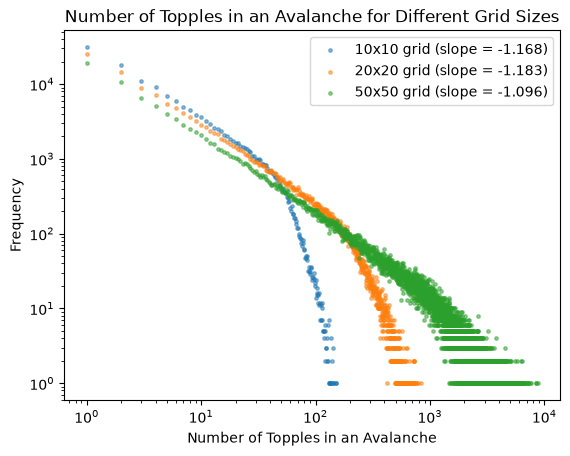
\includegraphics[width=0.8\linewidth]{figures/topplesgrid.png}
    \caption{The number of topples for the base model. The graph has a linear section, so we do observe scale-invariance in the number of topples.}
    \label{fig:topplesgrid}
\end{figure}

\begin{figure}
    \centering
    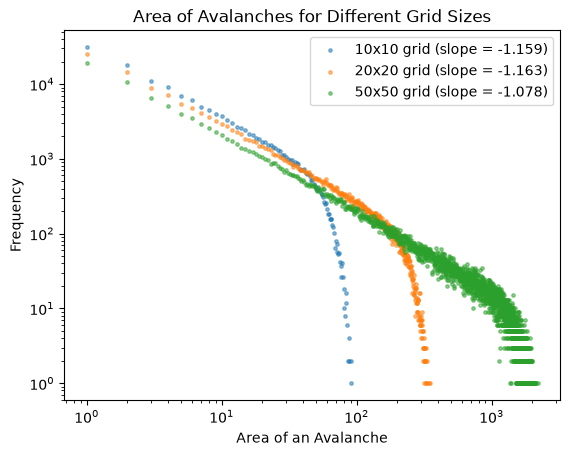
\includegraphics[width=0.8\linewidth]{figures/areagrid.png}
    \caption{The area of avalanches for the base model. The graph has a linear section, indicating that there is scale-invariance in the area of avalanches.}
    \label{fig:areagrid}
\end{figure}

\begin{figure}
    \centering
    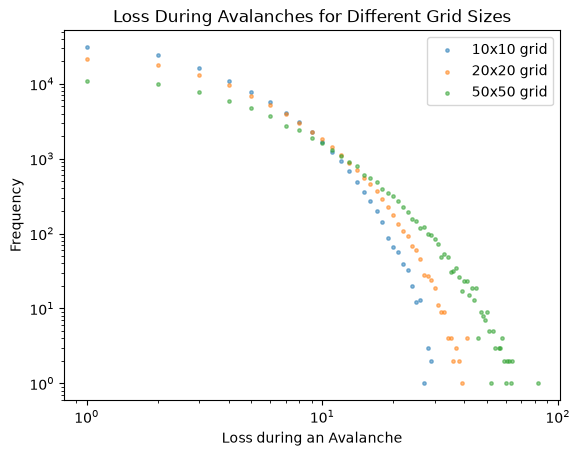
\includegraphics[width=0.8\linewidth]{figures/lossgrid.png}
    \caption{The loss for the base model. The graph is non-linear, indicating that loss does not follow a power law.}
    \label{fig:lossgrid}
\end{figure}

\begin{figure}
    \centering
    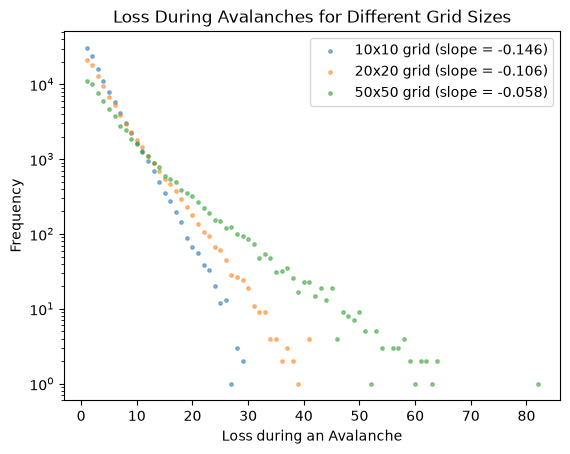
\includegraphics[width=0.8\linewidth]{figures/lossgrid2.png}
    \caption{The loss for the base model, now with only the frequency axis being in logarithm. The graph has a linear section, indicating that loss may follow an exponential relationship.}
    \label{fig:lossgrid2}
\end{figure}

\begin{figure}
    \centering
    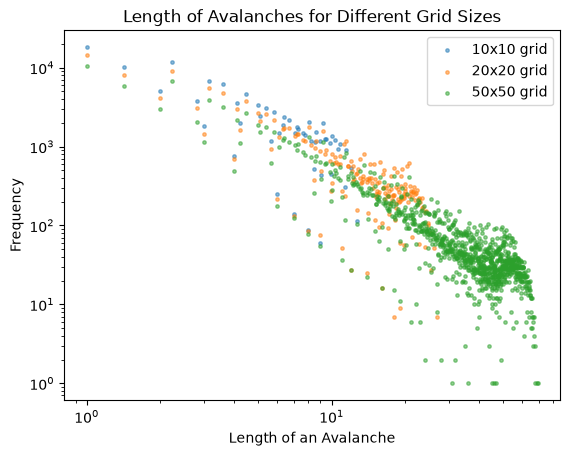
\includegraphics[width=0.8\linewidth]{figures/lengthgrid.png}
    \caption{The length of avalanches for the base model. The graph is linear but with a lot of variance.}
    \label{fig:lengthgrid}
\end{figure}



\newpage
\begin{question}
    Verify whether there was any correlation between the four properties we are recording for the avalanche.
\end{question}

\begin{table}[htbp]
    \centering
    \caption{Correlation matrices of avalanche statistics.}
    \label{tab:corr}
    \begin{tabular}{lrrrr}
        \toprule
         & Topples & Area & Loss & Length \\
        \midrule
        \multicolumn{5}{c}{$10 \times 10$ grid} \\
        \midrule
        Topples & 1.000000 & 0.985934 & 0.768923 & 0.897798 \\
        Area    & 0.985934 & 1.000000 & 0.774378 & 0.929118 \\
        Loss    & 0.768923 & 0.774378 & 1.000000 & 0.714528 \\
        Length  & 0.897798 & 0.929118 & 0.714528 & 1.000000 \\
        \midrule
        \multicolumn{5}{c}{$20 \times 20$ grid} \\
        \midrule
        Topples & 1.000000 & 0.968383 & 0.732303 & 0.860467 \\
        Area    & 0.968383 & 1.000000 & 0.734632 & 0.923382 \\
        Loss    & 0.732303 & 0.734632 & 1.000000 & 0.674210 \\
        Length  & 0.860467 & 0.923382 & 0.674210 & 1.000000 \\
        \midrule
        \multicolumn{5}{c}{$50 \times 50$ grid} \\
        \midrule
        Topples & 1.000000 & 0.936545 & 0.749283 & 0.802449 \\
        Area    & 0.936545 & 1.000000 & 0.727887 & 0.916770 \\
        Loss    & 0.749283 & 0.727887 & 1.000000 & 0.650059 \\
        Length  & 0.802449 & 0.916770 & 0.650059 & 1.000000 \\
        \bottomrule
    \end{tabular}
\end{table}


In Table~\ref{tab:corr}, we see that there was, in fact, positive correlation between each pair of statistics for each size grid. The correlation is strongest between topples and area, and weakest between length and loss. We see the strength of the correlation generally decreases as grid size increases, with the correlation between topples as loss being an exception to this as it increases from the 20x20 grid to the 50x50 grid..



\begin{question}
    Compare your initial expectation for the average height to what your simulation does. 
\end{question}


We measure the average height of the pile over 100,000 time steps (with a burn-in period) for a 10x10 grid, a 20x20 grid, and a 50x50 grid.

\begin{verbatim}
The average height for a 10x10 grid is: 2.006391836734694
The average height for a 20x20 grid is: 2.061899456521739
The average height for a 50x50 grid is: 2.097251712
\end{verbatim}

We see that the average height ranges from $2.01$ to $2.10$ depending on the grid size, with a larger grid having a larger average height. This agrees with our hypothesis. Simulating larger grids would be required to get closer to the limit of $2.125$ given by Caracciolo and Sportiello \cite{Car12}.


\section{Analysis of the extended model}

We now consider how changing the number of grains dropped at each time period changes the statistics. In Figure~\ref{fig:topplesdrop}, we see that the number of topples still maintains this power law relationship. Further, the gradient increases as the number of grains increases, possibly approaching a constant relationship. We note that our slope-fitting function fails to fit the case when $10$ grains are being dropped. The issue is with using the $R^2$ value to fit a function approaching a constant. If we consider how $R^2$ is defined, 
\[R^2=1-\frac{SS_{res}}{SS_{tot}}\]
it is clear that as the data approaches a constant, an $R^2$ value will approach 0. To fit a line in this case, we would need to use another method of measuring fit. For the area, we see a similar pattern in Figure~\ref{fig:topplesdrop}. 

We again use an exponential fit in Figure~\ref{fig:lossdrop2} for the loss statistic. As the number of grains increases, it appears that the relationship does not follow an exponential for small values of loss. As we have defined it, the length of an avalanche, seen in Figure~\ref{fig:lengthdrop}, does not follow a power law for larger numbers of dropped grains. This is because grains dropped far apart on the lattice can result in an avalanche which starts in multiple places, making the length values artificially large.



\begin{figure}
    \centering
    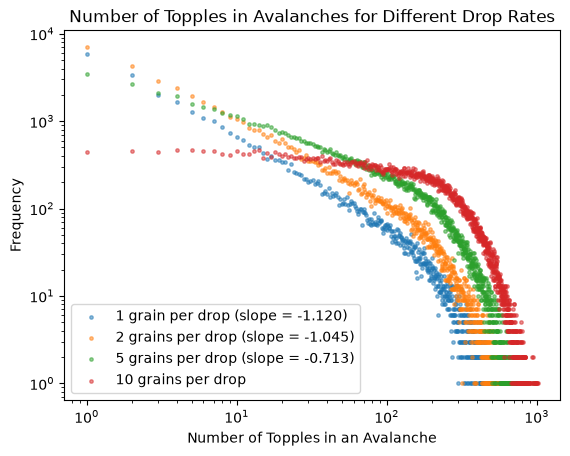
\includegraphics[width=0.8\linewidth]{figures/topplesdrop.png}
    \caption{The number of topples for the extension model. The gradients of the graphs increase as the number of grains increases.}
    \label{fig:topplesdrop}
\end{figure}

\begin{figure}
    \centering
    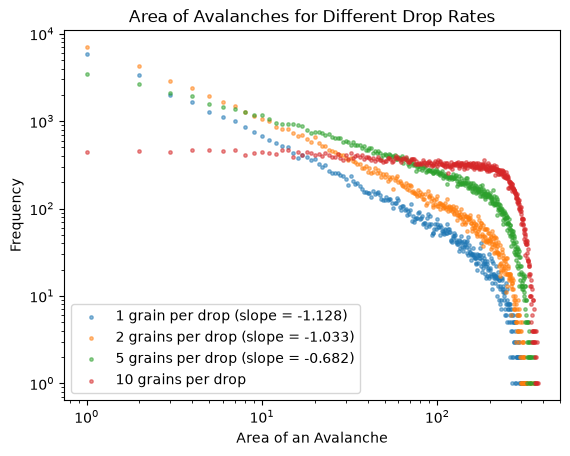
\includegraphics[width=0.8\linewidth]{figures/areadrop.png}
    \caption{The area of avalanches for the extension model. The gradients of the graphs increase as the number of grains increases.}
    \label{fig:areadrop}
\end{figure}

\begin{figure}
    \centering
    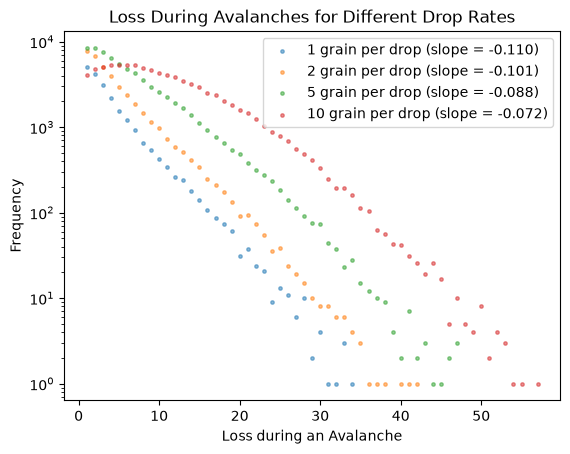
\includegraphics[width=0.8\linewidth]{figures/lossdrop2.png}
    \caption{The loss for the extension model, with only frequency having a log axis. The graphs have linear segments, indicating there is an exponential relationship. For small numbers of loss, the graph is non-linear, especially so for the larger number of drops.}
    \label{fig:lossdrop2}
\end{figure}

\begin{figure}
    \centering
    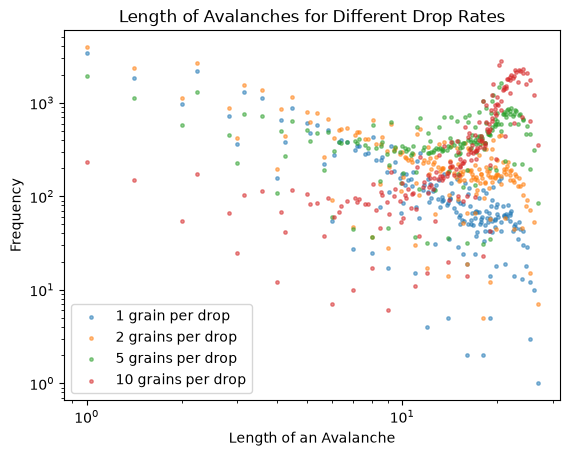
\includegraphics[width=0.8\linewidth]{figures/lengthdrop.png}
    \caption{The length of avalanches for the extension model. The graphs are clearly non-linear when more grains are dropped.}
    \label{fig:lengthdrop}
\end{figure}



\section{Conclusion}

To conclude, we see clear signs of \soc\ in the \btw\ model through the avalanche-topple and avalanche-area distributions. We also saw that the average height of the grid increased with grid size, approaching the known theoretical limit of $2.125$. Further, all four avalanche statistics showed pairwise correlation. When multiple grains were added simultaneously, the topples and area distributions continued to exhibit power-law behaviour, although their fitted slows were varying. In contrast, the loss and length distributions varied as the number of grains added changed, highlighting how the way the system is driven can influence the form of these statistics. Overall, the results demonstrate how complex behaviour can arise from the simple \btw\ model.